\documentclass{article}
\usepackage[utf8]{inputenc}
\usepackage[a4paper, total={6.5in, 9.5in}]{geometry}
\usepackage{float}
\usepackage{amsmath}
\usepackage{amssymb}
\usepackage{mathtools}
\usepackage{tensor}
\newcommand{\torseur}[7]{
\tensor[_{#1}]{\left\{ \begin{array}{cc}
  #2 & #5 \
  #3 & #6 \
  #4 & #7
\end{array} \right\}}{_{(\vec{x};\vec{y};\vec{z})}}
}
\usepackage{siunitx}
\sisetup{output-decimal-marker={,},group-minimum-digits=4,abbreviations}
\sisetup{inter-unit-product=\ensuremath{{}\cdot{}}}
\newcommand{\deftable}[2]{%
%\hline
\textbf{B.A.M.E}
\begin{table}[h]
  \centering
  \begin{tabular}{llp{130mm}}%
    %& unité/type & Explication \ \hline
    #1
  \end{tabular}
  \label{tab:#2_units}
\end{table}%
}
\newcommand{\deftablevar}[3]{%
  $#1$ & $\si{#2}$ & #3 \
}
\newcommand{\deftableobj}[3]{%
  $#1$ & \textit{#2} & #3 \
}
\newcommand{\bame}[1]{%
%\hline
\begin{table}[h]
  \centering
  \begin{tabular}{llllp{130mm}}%
    Nom & Vecteur & Direction & Sens & Norme \hline
    #1
  \end{tabular}
\end{table}%
}
\newcommand{\vect}[1]{\overrightarrow{#1}}

\title{Distribuer l'énergie}
\author{Ewen Le Bihan}
\date{2020-03-27}

\begin{document}

\maketitle

\section{}

Je n'ai pas réussi à extraire les informations du schéma de circuit

\section{}

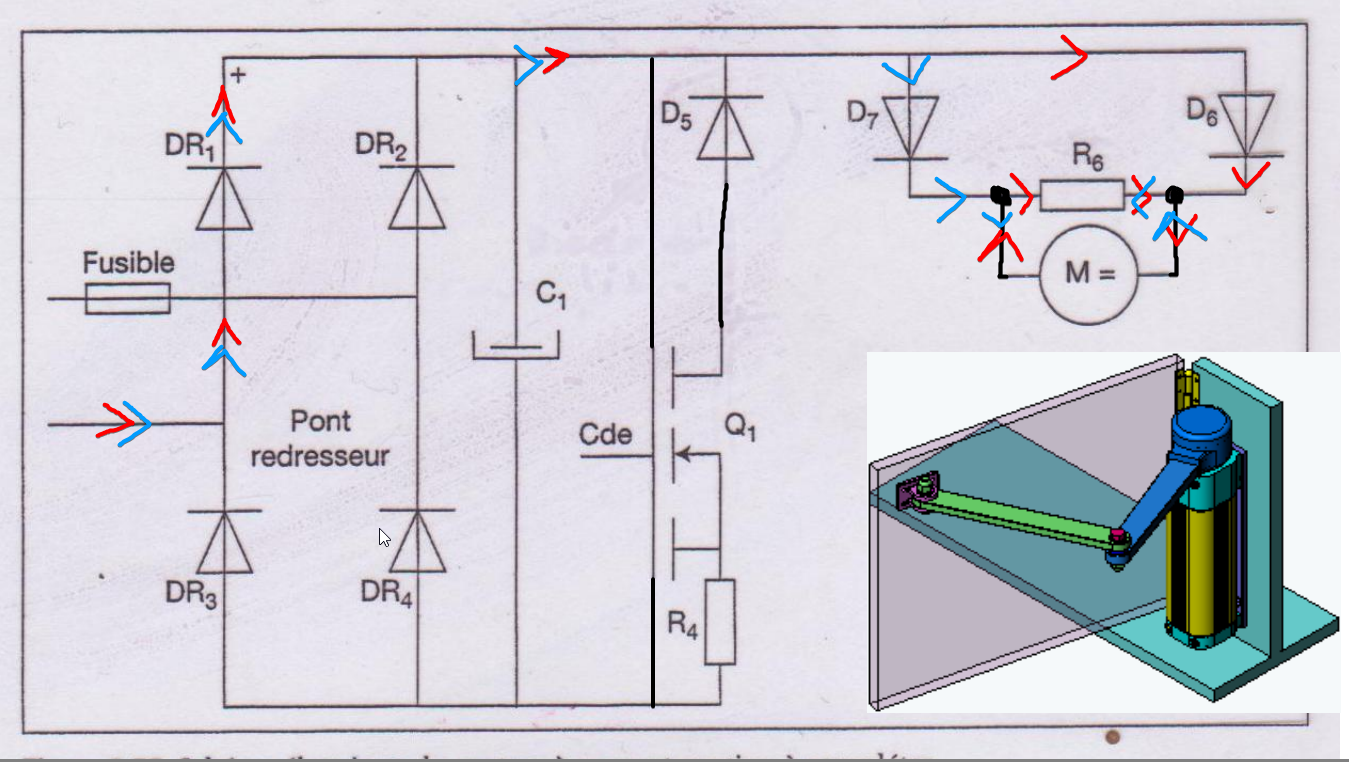
\includegraphics[width=15cm]{exo2.png}

\section{}

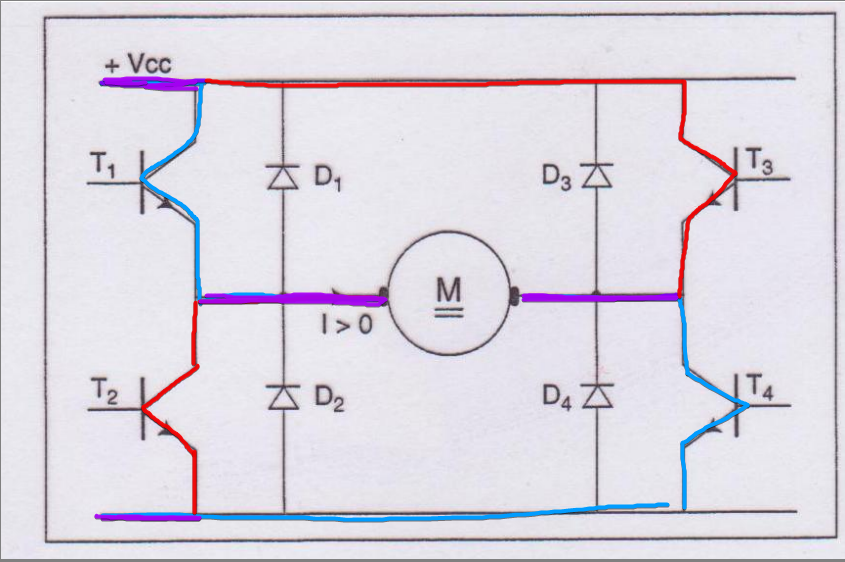
\includegraphics[width=15cm]{exo3.png}


\section{}
\subsection{}

\subsubsection{À \SI{45}{\kilo\meter\per\hour}}

$$\frac{0.8\cdot100}{60} = \SI{1.3}{\hour}$$

\subsubsection{À \SI{30}{\kilo\meter\per\hour}}

$$\frac{0.9\cdot100}{60} = \SI{1.5}{\hour}$$

\subsection{}

$$\frac{33}{60} = 0.55$$

\end{document}
